\documentclass[twoside,fancyhdr]{18_format/csethesis}
%\documentclass{18_format/iitgthesis}
\pdfminorversion=7
\listfiles
%\usepackage[unit=cm,showframe=true,color=red]{fgruler} %%% Add rular to pages
%\usepackage{showframe}
\usepackage{xcolor}
\usepackage{eso-pic}
\usepackage{transparent}
\usepackage{tikz}
\usepackage{lipsum}
\usepackage{fancyhdr}
%\usepackage[inner=3cm,outer=1cm,top=3cm,bottom=3cm,footskip=1cm]{geometry}
\usepackage[marginparwidth=0.0cm,top=4cm,inner=4cm,outer=3cm,bottom=4cm,head=23pt]{geometry}
%\usepackage{geometry}
%\usepackage{hyperref}
\usepackage{wrapfig, blindtext}
\usepackage{pdfpages}
\usepackage{graphicx}
%\DeclareGraphicsExtensions{.eps}
%\usepackage{caption}
\usepackage{subcaption}
%\usepackage{setspace}
%\captionsetup{font={small,stretch=0.80}}
\usepackage{epstopdf}
%\usepackage[linesnumbered,ruled,vlined,boxed]{algorithm2e}
\usepackage[linesnumbered,ruled,vlined,boxed]{algorithm2e}
	\newcommand\mycommfont[1]{\footnotesize\ttfamily\textcolor{blue}{#1}}
	\SetCommentSty{mycommfont}
\usepackage[fleqn]{amsmath}
\usepackage{amssymb}
\usepackage{multirow}
\usepackage{enumerate}
\usepackage{mathrsfs}
\usepackage{color}
\usepackage{float}
\usepackage{framed}
%\usepackage{cite}
\usepackage{tikz}
%\usepackage{breqn}
\usepackage{mathtools}
\usepackage{xifthen}
\usepackage{cases}
\usepackage{url}
\usepackage{algorithmic}
%\usepackage{qtree}
\usepackage{empheq}
%\usepackage [pagewise]{lineno}
\usepackage{enumitem}
\usepackage{listings}
\usepackage{color, colortbl}
%\usepackage[resetlabels]{multibib}
\usepackage[labelnumber, maxbibnames=99,defernumbers=true,style=numeric,backend=bibtex,maxcitenames=50, sorting=none]{biblatex}
\usepackage{imakeidx}
    \makeindex
    \makeindex[name=term,title={Terminologies}]
\usepackage[intoc]{nomencl}\makenomenclature
%\setnomtableformat{|l|l|}
\usepackage[printonlyused]{acronym}
\usepackage{xargs}
%\usepackage[paper=A4]{typearea}
\usepackage{afterpage}
\usepackage{pdflscape}
\usepackage{shadowtext}
\usepackage{etoolbox}
\usepackage{lineno}
\usepackage{afterpage}
\usepackage{multicol}
\usepackage{multirow}
\usepackage{comment}
%\usepackage{scrextend}
%\usepackage[english]{babel}
\usepackage[bookmarks=true]{hyperref}
\usepackage{bookmark}
\usepackage{adjustbox}
\usepackage{pdfpages}
%\setlist[description]{style = multiline, labelwidth = 40pt}
%%%%%%%%%%%%%%%%%%%%%%%%%%%%%%%%%%%%%%%%%%%%%%%%%%%%%%%%%
%=============================================================================
% SEGREGATE THE BIBLIOGRAPHY
%=============================================================================
%\newcites{th}{Publications Related to Thesis}
%\newcites{gen}{Other Publications of the Author}
\addbibresource{20_bibilography/ref-article.bib}
\addbibresource{20_bibilography/ref-proc.bib}
\addbibresource{20_bibilography/ref-oth.bib}
%\addbibresource{20_bibilography/total6.bib}
%\addbibresource{20_bibilography/new.bib}
\addbibresource{20_bibilography/mypub.bib}
%%%%%%%%%%%%%%%%
\DeclareCiteCommand{\citenum}
  {}
  {\printfield{labelnumber}}
  {}
  {}
%%%%%%%%%%%%%%%%  
\defbibenvironment{mypubs}
  {\enumerate[label={[T.\arabic*]}]
     {}
     {\setlength{\labelwidth}{\labelnumberwidth}%
      \setlength{\leftmargin}{\labelwidth}%
      \setlength{\labelsep}{\biblabelsep}%
      \addtolength{\leftmargin}{\labelsep}%
      \setlength{\itemsep}{\bibitemsep}%
      \setlength{\parsep}{\bibparsep}}%
      \renewcommand*{\makelabel}[1]{\hss##1}}
  {\endenumerate}
  {\item}
%%%%%%%%%%%%%%%%
\defbibenvironment{mypuboth}
  {\enumerate[label={[O.\arabic*]}]
     {}
     {\setlength{\labelwidth}{\labelnumberwidth}%
      \setlength{\leftmargin}{\labelwidth}%
      \setlength{\labelsep}{\biblabelsep}%
      \addtolength{\leftmargin}{\labelsep}%
      \setlength{\itemsep}{\bibitemsep}%
      \setlength{\parsep}{\bibparsep}}%
      \renewcommand*{\makelabel}[1]{\hss##1}}
  {\endenumerate}
  {\item}
%%%%%%%%%%%%%%%%%%%%%%%%%%%%%%%%%%%%%%%%%%%%%%%%%%%%%%%%%
\usepackage[capitalize]{cleveref}
%%%%%%%		Enable subsubsection numbering		%%%%%%%
\setcounter{tocdepth}{3}
\setcounter{secnumdepth}{3}
\renewcommand\thesubsubsection{\alph{subsubsection}}
%%%%%%%%%%%%%%%%%%%%%%%%%%%%%%%%%%%%%%%%%%%%%%%%%%%%%%%%%%%%%%%%%
%====== For Cover page
\definecolor{coverfont}{RGB}{255, 255, 255}  %White
\definecolor{covercolor}{HTML}{D4A138}
%\newcommand\crule[3][black]{\textcolor{#1}{\rule{#2}{#3}}}
\newcommand{\mycbox}[3]{\tikz{\path[draw=#1,fill=#1,rounded corners=10pt] (0,0) rectangle (#2,#3);}} 
%%%%%%%		For Code listing		%%%%%%%
\definecolor{codegreen}{rgb}{0,0.6,0}
\definecolor{codegray}{rgb}{0.5,0.5,0.5}
\definecolor{codepurple}{rgb}{0.58,0,0.82}
\definecolor{backcolour}{rgb}{0.95,0.95,0.92}

\lstdefinestyle{mystyle}{
    backgroundcolor=\color{backcolour},
    commentstyle=\color{codegreen},
    keywordstyle=\color{magenta},
    numberstyle=\tiny\color{codegray},
    stringstyle=\color{codepurple},
    basicstyle=\footnotesize,
    breakatwhitespace=false,         
    breaklines=true,                 
    captionpos=b,                    
    keepspaces=true,                 
    numbers=left,                    
    numbersep=5pt,                  
    showspaces=false,                
    showstringspaces=false,
    showtabs=false,                  
    tabsize=2
}
\lstset{style=mystyle}
%%%%%%%%%%%%%%%%%%%%%%%%%%%%%%%%%%%%%%%%%%%%%%%%%%%%%%%%%%%%%%%%
\newcommand{\nosemic}{\renewcommand{\@endalgocfline}{\relax}}% Drop semi-colon ;
\newcommand{\dosemic}{\renewcommand{\@endalgocfline}{\algocf@endline}}% Reinstate semi-colon ;
\newcommand{\pushline}{\Indp}% Indent
\newcommand{\popline}{\Indm\dosemic}% Undent
\let\oldnl\nl% Store \nl in \oldnl
\newcommand{\nonl}{\renewcommand{\nl}{\let\nl\oldnl}}% Remove line number 
%%%%%%%%%%%%%%%%%%%%%%%%%%%%%%%%%%%%%%%%%%%%%%%%%%%%%%%%%%%%%%%%
\newcommand\blfootnote[1]{%
  \begingroup
  \renewcommand\thefootnote{}\footnote{#1}%
  \addtocounter{footnote}{-1}%
  \endgroup
}
%%%%%%%%%%%%%%%%%%%%%%%%%%%%%%
\providecommand{\fullcitenum}[1]{[T.\citenum{#1}] \fullcite{#1}}
\providecommand{\Othcite}[1]{[O.\citenum{#1}]}
%%%%%%%%%%%%%%%%%%%%%%%%%%%%%%
\newtheorem{question}{Question}[section]
%%%%%%%%%%%%%%%%%%%%%%%%%%%%%%%%%%%%%%%%%%%%%%%%%%%%%%%%%%%%%%%%%%%%%%%%%%%%%%%%%%%%%%%%%%%%%%%%
%%%%%%%		Beamer Only		%%%%%%%
\providecommand{\figtext}[1]{{\fontsize{30}{30}\selectfont #1}}
\providecommand{\reducecounter}[1]{%
\ifthenelse{\equal{#1}{}}{\addtocounter{framenumber}{-1}}{\addtocounter{framenumber}{-#1}}%
}
%%%%%%%%%%%%%%%%%%%%%%%%%%%%%%%%%%%%%%%%%%%%%%%%%%%%%%%%%%%%%%%%%%%%%%%%%%%%%%%%%%%%%%%%%%%%%%%%
%%%%%%%		Paper Only		%%%%%%%
\crefname{appsec}{Appendix}{Appendices}
\crefname{algocf}{Alg.}{Algs.}
\Crefname{algocf}{Algorithm}{Algorithms}
\Crefname{chapter}{Chapter}{Chapters}
\Crefname{subequation}{Sub-eq.}{Sub-eqs.}
\crefname{subequation}{sub-eq.}{sub-eqs.}
\newcommand{\csubref}[1]{\namecref{#1}~(\ref{#1})}
\newcommand{\pairsum}{\mathbin{\ooalign{$\circ$\cr$\sum$\cr}}}
%\newcounter{problemCounter}[section]
\crefname{problem}{Problem}{Problems}
%\newenvironment{problem}[1][]{\refstepcounter{problemCounter}\par\medskip
%   \noindent \textbf{Problem~\theproblemCounter} \rmfamily}{\medskip}
%%%%%%%%%%%%%%%%%%%%%%%%%%%%%%%%%%%%%%%%%%%%%%%%%%%%%%%%%%%%%%%%%%%%%%%%%%%%%%%%%%%%%%%%%%%%%%%%
%%%%%%%		For all		%%%%%%%
\providecommand{\etal}{\emph{et.al.}}
\providecommand{\noteS}[1]{\textcolor{blue}{Subho: #1}}
\providecommand{\notesu}[1]{\textcolor{blue}{Subho: #1}}
\providecommand{\notesc}[1]{\textcolor{red}{Sandip: #1}}

\providecommand{\redtext}[1]{\todo[color=blue!20]{#1}}
\newcommand{\textuparrow}{\cellcolor{blue!20}\textbf{$\uparrow$}}
\newcommand{\textleftarrow}{\cellcolor{blue!20}\textbf{$\leftarrow$}}
%%%%%%%%%%%%%%%%%%%%%%%%%%%%%%%%%%%%%%%%%%%%%%%%%%%%%%%%%%%%%%%%%%%%%%%%%%%%%%%%%%%%%%%%%%%%%%%%
%\newcommand{\authorMe}{Chattopadhyay, Subhrendu}
%%%%%%%%%%%%%%%%%%%%%%%%%%%%%%%%%
\newcommand{\iflabelexists}[3]{\ifcsundef{r@#1}{#3}{#2}}
%%%%%%%
\providecommand{\paperName}[1]{\texttt{#1}}
%%%% 
%%		Wrapper acronym with index commands
%%%%
\providecommand{\addac}[2][]{%\addac[RTT]{Round Trip Time} OR \addac{RTT}
    \ifthenelse{\equal{#1}{}}%
    {\ac{#2}\index{\acs{#2}}}% Single Arg
    {\acrodef{#1}{#2}\ac{#1}\index{#1}\index{#2|seealso{#1}}}}
%%%%%%%    
\providecommand{\addacp}[1]{\acp{#1}\index{\acs{#1}}}
%%%%%%%
%\providecommand{\addacm}[3]{\acrodef{#1}[#2]{#3}\ac{#1}\index{#3|seealso{#2}}\index{#2}}
%\providecommand{\term}[1]{``\textit{#1}''\index{#1}}
%%%%%%%%
\providecommand{\firstOcc}[1]{
	\acf{#1} \index{\acl{#1}} \index{\acl{#1}|seealso{\acs{#1}}}}
%%%%%%%
\providecommand{\termit}[1]{\addTerm{\textit{#1}}}
\providecommand{\termtt}[1]{\addTerm{\texttt{#1}}}
\providecommand{\addTerm}[1]{``\emph{#1}"\index{\normalfont{#1}}}
%%%%%%%
%\providecommand{\termtt}[2][]{%\term[RTT]{Round Trip Time} OR \term{RTT}
%\ifthenelse{\equal{#1}{}}%
%    {\texttt{\acs{#2}}\index{\acs{#2}}}
%    {\texttt{\addac[#1]{#2}}\index{#1}\index{#2|seealso{#1}}}
%%%%%%%
%\providecommand{\termit}[2][]{%\term[RTT]{Round Trip Time} OR \term{RTT}
%    \ifthenelse{\equal{#1}{}}%
%    {\textit{\acs{#2}}\index[term]{\acs{#2}}}
%    {\textit{\addac[#1]{#2}}\index{#1}\index{#2|seealso{#1}}}}
%%%%%%%
%\providecommand{\term}[2][]{%\term[RTT]{Round Trip Time} OR \term{RTT}
%\ifthenelse{\equal{#1}{}}%
%    {``\termit{#2}''}% Single Arg
%    {``\termit[#1]{#2}"}}
%%%%%%%%

%%%%%%%%%%%%%%%%%%%%%%%%%%%%%%%%%%%%%%%%%%%%%%%%%%%%%%%%%%%%%%%%
\newcommand*\circled[1]{\tikz[baseline=(char.base)]{
            \node[shape=rectangle,draw,inner sep=2pt] (char) {#1};}}
%%%%%%%%%%%%%%%%%%%%%%%%%%%%%%%%%%%%%%%%%%%%%%%%%%%%%%%%%%%%%%%%
%\DeclareFieldFormat{labelnumberwidth}{\mkbibbrackets{#1}}
%\renewbibmacro*{cite}{%
%  \printtext[bibhyperref]{%
%    \printfield{labelprefix}%
%    \ifkeyword{secondary}
%      {\printfield{labelnumber}}
%      {\printfield{labelalpha}%
%       \printfield{extraalpha}}}}
%
%\defbibenvironment{bibliographyNUM}
%  {\list
%     {\printtext[labelnumberwidth]{%
%        \printfield{labelprefix}%
%        \printfield{labelnumber}}}
%     {\setlength{\labelwidth}{\labelnumberwidth}%
%      \setlength{\leftmargin}{\labelwidth}%
%      \setlength{\labelsep}{\biblabelsep}%
%      \addtolength{\leftmargin}{\labelsep}%
%      \setlength{\itemsep}{\bibitemsep}%
%      \setlength{\parsep}{\bibparsep}}%
%      \renewcommand*{\makelabel}[1]{\hss##1}}
%  {\endlist}
%  {\item}
%%%%%%%%%%%%%%%%%%%%%%%%%%%%%%%%%%%%%%%%%%%%%%%%%%%%%%%%%
%\def\macro{Modular and Response}
%%%%%%%%%%%%%%%%%%%%%%%%%%%%%%%%%%%%%%%%%%%%%%%%%%%%%%%%%
%\linenumbers
%\usepackage{style/qtree}
%%%%%%%%%%%%%%%%%%%%%%%%%%%%%%%%%%%%%%%%%%%%%%%%%%%%%%%%%
\phdtitle = {{SDN for Large Scale IoT Networks}} % { and } are needed around your name
%\phdtitle = {{Light-weight Self-stabilizing Dynamic NIB Placement For Distributed Large Scale SDN}}
\name = {Subhrendu Chattopadhyay}          % and other fields. don't remove.
\rollno = {146101002}
\guide = {Prof. Sukumar Nandi}
%%%%%%%%%%%%%%%%%%%%%%%%%%%%%%%%%%%%%%%%%%%%%%%%%%%%%%%%%%%%%%%%%
\begin{document}
  %%%% Front Cover Page
  \pagenumbering{alph}
  \pdfbookmark{Front Cover}{Front Cover}
  %%============================================================================
%% FrontCoverPage
%%===========================================================================
%\pagenumbering{roman}
%%\chapter*{}
%\thispagestyle{empty}
%%\pagecolor{covercolor}
%\color{coverfont}
%\newgeometry{margin=0pt}
%%\pagecolor{covercolor} % Cover color defined in \17_Util/newcommands.tex
%%\begin{center}
%%\begin{overpic}[width=.99\paperwidth]{0-cover/ThesisTopCover.png}% add grid to options for positioning
%%Adjust title position by changing \put (x,y)
% %\put(0,0){A} \put(67,99){B}
%% \put (0,86){\transparent{0.8}\mycbox{black}{17cm}{3cm}} % background boxes
%% \put (4,90) {\begin{minipage}{0.7\linewidth} \huge\sf\textbf{\the\phdtitle}\end{minipage}}
%% \put (24,16){\transparent{0.8}\mycbox{black}{13cm}{3cm}} % background boxes
%% \put(29,21){{\LARGE{\textbf{\textit{\the\name}}}}}
%%\end{overpic} 
%%\end{center}
%%\cleardoublepage
%\pagecolor{white}
%%\cleardoublepage
%\color{black}
%\restoregeometry
%============================================================================
% FrontCoverPage
%===========================================================================
\pagenumbering{roman}
%\chapter*{}
\thispagestyle{empty}
\textheight 16in \textwidth 12.5in {\huge\sf  \textbf{\the\phdtitle}}\\[100ex]

\begin{flushright}
\LARGE{\textbf{\textit{\the\name}}}
\end{flushright}
%\cleardoublepage

%  \includepdf[pages={2}]{C0_Cover.pdf}
  %\linenumbers
    \clearpage  
  %\blankpage
  %\startOddPage
  \pagenumbering{roman}
  \pdfbookmark{Title Page}{Title Page}
  \newgeometry{margin=0pt}
\chapter*{}
\pagenumbering{roman}
\thispagestyle{empty}
%\begin{titlepage}
\begin{center}
%\textheight 5in \textwidth 12.5in {\huge\sf  \textbf{  }}\\[5ex]
\textheight 16in \textwidth 12.5in {\huge\sf  \textbf{\the\phdtitle}}\\[20ex]
{\Large{\textit{
%{\Large \bf Synopsis Report}\\
{Thesis submitted in partial fulfilment \\of the requirements
for the degree of\\
[5ex]{\Large \bf Doctor of Philosophy}
}}}}\\
[5ex] \large\emph{by} \\[1ex]
{\sf \sf \Large\bf{\the\name}}\\[5ex]
\large\textit{under the supervision of}\\[2ex]
{\Large \bf \the\guide} \\[5ex]

%\vspace{.05in}
 \begin{figure}
    \begin{minipage}{\linewidth}
      \centering
      
\includegraphics[scale=.9]{0-title/iitg_logo}
    \end{minipage} 
  \end{figure}

%{\sl \bf{to the}} \\[1ex]
{\large \bf Department of Computer Science and Engineering}  \\[1ex]
{\Large \bf{INDIAN INSTITUTE OF TECHNOLOGY GUWAHATI \\GUWAHATI - 781039, INDIA}}\\
{\large\bf {\today}}
\end{center}
\restoregeometry

  \startOddPage
  %\pagenumbering{roman}
\thispagestyle{plain}
\chapter*{}
  \pdfbookmark{Dedication}{Dedication}
\vskip 1.5cm
\dedication
    \begin{figure}[!ht]
        \centering
        \begin{minipage}{\textwidth}
            \centering
            \includegraphics[clip, trim=0 250 20 0, width=\textwidth]{0-certificate/Quote.pdf}
        \end{minipage}
    \end{figure}
    \textbf{\textit{\Large{``The absolute knowledge can be attained after thinking, reasoning and assimilation''}}} \\[10ex]
    \textbf{\textit{\Huge{Dedicated to}}}\\[3ex]
   \textbf{\textit{\Huge{All my teachers}}}\\[3ex]
   \normalsize{\it Who taught me to assimilate the information to convert it into knowledge.}
   \clearpage
\enddedication
%\startOddPage
%%%%%%%%%%%%%%%%%%%%%%%%%%%%%%%%%%%%%%%%%%%%%%%%%%%%%%%%%%%%%%%%%%%%%%%%%%%%%%%%%%%%
%\raggedbottom
%\thispagestyle{empty}
\chapter*{\centering Declaration}
  \pdfbookmark{Declarations}{Declarations}
%\begin{Declaration}
 I declare that
 \begin{enumerate}
  \item The work contained in this thesis is original and has been done by myself under the general supervision of my supervisor.
  \item The work has not been submitted to any other Institute for any degree or diploma.
  \item Whenever I have used materials (data, theoretical analysis, results) from other sources, I have given due credit to them by citing them in the text of the thesis and giving their details in the references.
  \item Whenever I have quoted written materials from other sources, I have put them under quotation marks and given due credit to the sources by citing them and giving required details in the references. 
 \end{enumerate}
\vspace{2cm}
%\begin{flushright}
\begin{tabular}{p{.3\textwidth}l}
Place: IIT Guwahati  &\large \textbf{Subhrendu Chattopadhyay}\\
Date:  & Research Scholar\\
  & Department of Computer Science and Engineering, \\
  & Indian Institute of Technology Guwahati,\\
  & Guwahati, INDIA 781039
\end{tabular}
%\end{flushright}
%\end{Declaration}
%%%%%%%%%%%%%%%%%%%%%%%%%%%%%%%%%%%%%%%%%%%%%%%%%%%%%%%%%%%%%%%
\startOddPage
\chapter*{\centering Certificate}
%\begin{Certificate}
  \pdfbookmark{Certificates}{Certificates}
\vskip 2ex \quad This is to certify that the work contained
in this thesis entitled ``\the\phdtitle'' 
is a bonafide work of \the\name
(Roll No. \the\rollno), carried out in the Department of
Computer Science and Engineering, Indian Institute of Technology
Guwahati under my supervision and that it has not been submitted
elsewhere for a degree.

\vspace{2cm}
\begin{tabular}{p{.3\textwidth}l}
Place: IIT Guwahati & \large \textbf{\the\guide}\\
Date:  &Department of Computer Science and Engineering, \\
 & Indian Institute of Technology Guwahati,\\
 & Guwahati, INDIA 781039
\end{tabular}
%\end{Certificate}
%\clearpage
\startOddPage
  \clearpage  
  %\startOddPage
  \chapter*{\centering Acknowledgements}
\addcontentsline{toc}{chapter}{Acknowledgements}
\thispagestyle{cleanPage}
This thesis would not have been complete without the support of my thesis supervisor \textit{Prof. Sukumar Nandi} and my mentor \textit{Dr. Sandip Chakraborty}. Both of them have provided their support, knowledge and guidance to help me in my research. I have been working with both of them from my early days of M.Tech. I am truly grateful to them for putting me back in track during the trying times of my PhD. I have also learned many things about life while having a discussion with them. Their constant support and positive criticism have influenced my attitude, nature and personality in many ways.

I am very thankful to my doctoral committee members \textit{Prof. Diganta Goswami}, \textit{Prof. Ratnajit Bhattacharya} and \textit{Dr. Tamarapalli Venkatesh} for understanding my works and providing valuable comments to improve the work. I express my sincere thanks to former \textit{Head of the Department} \textit{Prof. S.B. Nair} and \textit{Prof. S.V. Rao} and current \textit{Head of the Department} \textit{Prof. Jatindra Deka} for providing a nice research environment in the \textit{Department of Computer Science and Engineering, IITG} and support my research work in many ways. During my early stages of research I enjoyed discussion with \textit{Dr. Sushanta Karmakar} and \textit{Dr. Arnab Sarkar} who helped and motivated me in a lot of ways. I am forever grateful for their support and time.

I am also very grateful to \textit{Tata Consultancy Services India Private Limited} for awarding me the research fellowship that gave me extremely good opportunities to broaden my research activities and interact with eminent researchers in the world, both from the industry as well from the academia. I thank \textit{Mr. Sachin Parkhi}, \textit{Program Manager of TCS Research Scholar Program}, for extending their helps and supports in technical and official activities. 

I had the privilege to collaborate with \textit{Dr. Sushanta Karmakar}, \textit{Dr. Samar Shailendra}, \textit{Prof. Soumya Kanti Ghosh} and \textit{Dr. Abhinandan S Prasad} whose interest and knowledge has enriched me a lot. I also enjoyed working with \textit{Dr. Niladri Sett}, \textit{Mr. Soumyajit Chatterjee} and \textit{Mr. Shubabrata Nath}. I express my sincere gratitude towards \textit{Mr. Debasish Naskar} for designing the logos and cover page of this thesis.

I would also like to express my hearty gratitude to \textit{Prof. Gautam Barua} and \textit{Prof. Gautam Biswas} the past Directors of the institute,  \textit{Prof. T. G. Sitharam} the present Director of the institute, all the Deans and other officials of IIT Guwahati, whose collective efforts have made this institute a place for world-class studies and research. I am thankful to all the faculties and the staffs of the Department of Computer science and Engineering for extending their cooperation in terms of technical and official supports. I thank the research scholars, M. Tech and the B. Tech students of this institute, with whom I have closely worked. I am sorry for not to mention all of their names, however, I have learned a lot from them during the course of our discussions.


I am forever thankful to \textit{Rahul, Soumadip, Akash, Mandar} and \textit{Ujjal} for the countless coffee sessions and round of discussions on various topics of interests which I will be missing in my upcoming days. My sincere thanks to my lab-mates \textit{Pranav, Madhurima, Pradeep, Debanjan, Kangan} and \textit{Sikha} for providing me a healthy work environment and helping me out during my needs. I am thankful to \textit{Bennith and Suraj} who helped me to develop experimentation frameworks.

Last, but not least, I probably would not have done a PhD were it not for my parents. From the childhood they have encouraged me to raise questions and indulged my curiosities. Many of the things I appreciate in research can be traced back to an idealized version of what my parents said while I was growing up. While, I often disagree with
them on issues, everything I do is influenced by them. My wife \textit{Piyali} also helped me in writing and proof reading this thesis. Her constant support has helped me a lot in writing this thesis.

Finally, there are several collaborators and anonymous reviewers who are not listed out explicitly, but who had an impact on my experience in grad school: people who enabled me to solve new problems, find new topics, and just meet new people. This acknowledgement was getting too long to list everyone, but know that all of you made a huge difference.

\vspace{2cm}
%\begin{flushright}
\begin{tabular}{p{.3\textwidth}p{.7\textwidth}}
Place: IIT Guwahati  & \large{ \centering \textbf{Subhrendu Chattopadhyay}}\\
Date:  & 
\end{tabular}
%\clearpage
%\end{acknowledgements}
%\newpage
  %%%%%%%%%%%%%%%%%%%%%%%%%%%%%%%%%%%%
  \chapter*{\centering Abstract}
\addcontentsline{toc}{chapter}{Abstract}
\thispagestyle{cleanPage}
\addac{IoT} is one of the rapidly growing network technologies which has the potential to serve millions of devices. Such \addac{LSN} requires network management to efficiently serve the end-user applications. Traditional Internet architecture suffers from lack of flexibility in the management of the network. The emergence of \addac{SDN} paradigm provides a flexible architecture for network control and management, in the cost of deploying new hardware by replacing the existing routing infrastructure. Further, the centralized controller architecture of \addac{SDN} makes the network prone to single point failure and creates the performance bottleneck. The scalability and failure prone nature of \addac{SDN} becomes the road block to employ \addac{SDN} in context of \addac{LSN}. The objective of this thesis is to design a distributed scalable \addac{SDN} orchestration framework which is suitable for handling the dynamic nature of\addac{LSN}. Additionally in this thesis we explore the performance improvement of \addac{IoT} applications by utilizing \addac{SDN}. 

Modern \addac{IoT} and hand-held devices are equipped with multiple interfaces. To leverage the bandwidth capacity of multiple interfaces several multi-path transport layer protocols exist which provides bandwidth aggregation. The first contribution in this thesis enhances the performance of \addac{IoT} applications by proposing \addac{SDN} control plane application \paperName{SDN-MPTCP} for \addac{MPTCP}, where \addac{MPTCP} is one of the popular multipath transport protocol. In this work we find that, \addac{MPTCP} performance has a strong correlation with the selected paths, and \addac{SDN} can assist in path selection of \addac{MPTCP}. In the next work, we investigate the \addac{SDN} deployment challenges for \addac{LSN}. As mentioned earlier, \addac{SDN} requires deployment of \addac{SDN} supported hardware, which can increase the \addac{capex} of \addac{SDN}. In this work we utilized \addac{NFV} for development of \paperName{FLIPPER}. \paperName{FLIPPER} enables deployment of \addac{SDN} like network management over existing \addac{COTS} devices of \addac{LSN} by converting them into \addac{PDEP}. \paperName{FLIPPER} provides a scalable, flexible, fail-safe and distributed \addTerm{self-stabilized} architecture. In the next contribution we use \paperName{FLIPPER} to design \paperName{Aloe} orchestration framework which utilizes the \addac{INP} platforms of \addac{LSN} to achieve \addTerm{servicification} of \addac{SDN} control plane. \paperName{Aloe} promises \addTerm{plug-and-play} and \addTerm{zero touch deployment} along with light-weight, fault-tolerant and auto-scalable network management platform for \addac{LSN}. Through exhaustive experimentation over an in-house test bed and \addac{AWS} platform we find that, \paperName{Aloe} can significantly improve performance of various \addac{IoT} applications. During this study we also observed that, various end-user applications targeted for \addac{LSN} require \addac{VNF} based \addac{SFC} depending on the network service access policy. However, dynamic deployment of \addacp{VNF} and traffic steering through those \addacp{VNF} to preserve the \addac{SFC} ordering is difficult in a \addac{LSN} which spans across multiple administrative domain. In the next contribution we propose \paperName{Amalgam} which incorporates \addac{SFC} management with \paperName{Aloe} to ensure scalability and dynamic \addac{SFC}. Based on the NP-hard nature of \addac{VNF} placement problem, \paperName{Amalgam} also proposes a greedy heuristic for \addac{VNF} placement which ensures fast flow initialization and provides performance improvement for short-duration flows. As a whole, this thesis provides auto-scalable, fault-tolerant and short-flow friendly distributed architecture and orchestration framework for \addac{LSN} network management to provide fine-grained network control.
  %%%%%%%%%%%%%%%%%%%%%%%%%%%%%%%%%%%%  
  \pdfbookmark{\contentsname}{Contents}
  \tableofcontents
  \cleardoublepage
  \listoffigures
  \cleardoublepage
  \listoftables
  \cleardoublepage
  \pdfbookmark{List of Algorithms}{List of Algorithms}
  \listofalgorithms
  \chapter*{List of Abbreviations}
  \addcontentsline{toc}{chapter}{List of Abbreviations}
  %\section*{Nomenclature}
\begin{multicols}{2}
	\begin{acronym}
		\acro{ACL}{Access Control Lists}
		\acro{API}{Application Programming Interfaces}
		\acro{AP}{Access Points}
		\acro{ARIMA}{Autoregressive Integrated Moving Average}
		\acro{ARP}{Address Resolution Protocol}
		\acro{AWS}{Amazon web service}
		\acro{BALIA}{Balanced Linked Increase Algorithm}
		\acro{BGP}{Border Gateway Protocol}
		\acro{COTS}{Commercial off-the-shelf}
		\acro{CTLR}{Controller State}
		\acro{DAL}{Device Abstraction Layer}
		\acro{DCN}{Data Center Networks}
		\acro{DD}{distributed database}
		\acro{DHT}{Distributed Hash Table}
		\acro{DHT-NIB}{Distributed Hash Table based NIB}
		\acro{DHT-flipper}{Distributed Hash Table based flipper}
		\acro{DNS}{Domain Name Server}
		\acro{DPI}{Deep Packet Inspector}
		\acro{DTMC}{Discrete Time Markov Chain}
		\acro{EWP}[element wise product]{Hadamard product}
		\acro{EM}{Element manager}
		\acro{EV}{Electric Vehicle}
		\acro{HOL}{Head of Line}
		\acro{ICN}{Information centric network}
		\acro{ID}{identifier}
		\acro{IoT}{Internet of things}
		\acro{IETF}{Internet Engineering Task Force}
		\acro{ISPN}{Internet Service Provider Network}
		\acro{l2tp}{Layer Two Tunneling Protocol}
		\acro{LIA}{Linked Increase Algorithm}
		\acro{LLDP}{Link Layer Discovery Protocol}
		\acro{LSA}{Linked State Advertisement}
		\acro{LAN}{Local area network}
		\acro{M2M}{Machine to Machine}
		\acro{MAPE}{Mean Average Percentage Error}
		\acro{MEC}{Mobile Edge Computing}
		\acro{MILP}{mixed integer linear program}
		\acro{MIS}{Maximal Indemendent Set}
		\acro{MPTCP}{Multipath TCP}
		\acro{NAT}{Network Address Translation}
		\acro{NFVI}{NFV infrastructure}
		\acro{NFVO}{NFV orchestrator}
		\acro{NFV}{Network Function Virtualization}
		\acro{NF}{Network Functions}
		\acro{NIB}{Network Information Base}
		\acro{NOS}{Network Operating System}
		\acro{NSAL}{Network Service Abstraction Layer}
		\acro{OS}{Operating System}
		\acro{OOS}{Out of order segments}
		\acro{ODL}{Open Day light}
		\acro{OFS}{OpenFlow supported switch}
		\acro{OLIA}{Opportunistic Linked Increase Algorithm}
		\acro{OVS}{Open virtual switch}
		\acro{P2NM}{PushToNode Module}
		\acro{PDEP}{Policy decision and enforcement point}
		\acro{PMM}{Path Manager Module}
		\acro{PRIO}{Priority}
		\acro{PSI}{Public subscribe internet}
		\acro{MPTCP}{Multipath TCP}
		\acro{QoS}{Quality of Service}
		\acro{RMM}{Resource Management Module}
		\acro{RE}{Resource Enforcer}
		\acro{RM}{Resource Monitor}
		\acro{REST}{REST API}
		\acro{RTT}{Round Trip Time}
		\acro{SCI}{Service Chain Identifier}
		\acro{SCM}{Service Chain Manager}
		\acro{SDC}{Service Deployment Controller}
		\acro{SDM}{State Discovery Module}
		\acro{SDN}{Software-Defined Network}
		\acro{SFC}{Service Function Chaining}
		\acro{SNC}{Super Network Controller}
		\acro{SNMP}{Simple Network Management Protocol}
		\acro{SS-MIS}{self-stabilizing MIS}
		\acro{STP}{Spanning Tree Protocol}
		\acro{SVM}{Support vector machine}
		\acro{TCP}{Transmission Control Protocol}
		\acro{TCAM}{Ternary Content-Addressable Memory}
		\acro{TFTP}{Trivial file Transfer Protocol}
		\acro{TMM}{Topology Management Module}
		\acro{VIM}{Virtualized infrastructure manager}
		\acro{VMM}{VNF manager module}
		\acro{VM}{Virtual Machines}
		\acro{VNFM}{VNF Manager}
		\acro{VNF}{Virtual Network Function}
		\acro{WAN}{Wide area network}
		\acro{capex}{capital expenditure}
		\acro{opex}{operational expenditure}
		\acro{pmf}{probability mass function}
		\acro{PSI}{Public subscribe internet}
		%%%%%%%%%%
		\acro{Rpi}{Raspberry Pi}
		\acro{e}[\ensuremath{e}]{Euler-Mascheroni constant}
		\acro{INP}[In-network processing]{in-network or In-network processing}
		\acro{LSN}[LSiN]{large scale IoT network}
		\acro{OSSBSS}[OSS/BSS]{Operations and Business Support Systems}
		\acro{US}[\ensuremath{\mu}S]{micro-service}
		\acro{UC}[\ensuremath{\mu}C]{micro-controller}
		\acro{UMM}[\ensuremath{\mu}MM]{\ensuremath{\mu}C Manager Module}
		\acro{UPM}[\ensuremath{\mu}PM]{\ensuremath{\mu}C Placement Module}
		\acro{ucaas}[\ensuremath{\mu}CaaS]{\ensuremath{\mu}C as a Service}
		\end{acronym}
\end{multicols}
%\DeclareAcronym{INP}{short = In-network processing ,long  = in-network or In-network processing}
%%%%%%%%%%%%%%%%%%%%%%%%%%%%%%%%%%%%%%%
\begin{comment}
\acro{POX}

\acro{UDP}
\acro{Amalgam}
\acro{Cassandra}
\acro{Gluster}
\acroit{MiniDockNet}
\acroit{Mininet}
\acroit{nano}


\acro{Barista}
\acro{Cassandra}


\acro{Ethernet}
\acro{FastRule}
\acro{GlusterFS}
\acro{Gluster}
\acro{HTTP}
\acro{ICMP}
\acro{JSON}

\acro{MP\

\acro{NoSQL}
\acro{OFPT\

\acro{OS}
\acro{OpenFlow}

\acro{REST}
\acro{RPC}
\acro{Raspbian}
\acro{Ryu}
\acro{SLAB}
\acro{STP}
\acro{SYN}
\acro{SimpleHTTPServer}
\acro{Swift}
\acro{TCAM}
\acro{TCP}
\acro{VLAN}
\acro{Zero}
\acro{atleast}
\acro{cassendra}
\acro{cgroups}
\acro{docker}
\acro{iperf}
\acro{packet\
\acro{ping}
\acro{python}
\acro{rocketfuel}
\acro{rpc}
\acro{steer}
\acro{tc}
\acro{Cloud}
\acro{DAL}
\acro{DCN}
\acro{Dysco}
\acro{FLIPPER}
\acro{Flipper}
\acro{INP}
\acro{ISPN}
\acro{MIS}
\acro{Markov}
\acro{Mininet}
\acro{ONIX}

\acro{OpenFlow}

\acro{Rpi}
\acro{TCP}
\acro{Things}


\acro{Winner}
\acro{\
\acro{acknowledgments}
\acro{anytime}
\acro{anywhere}
\acro{capex}
\acro{controllers}
\acro{controller}
\acro{firewall}
\acro{flipper}
\acro{flip}
\acro{flows}
\acro{flow}
\acro{heterogeneous}
\acro{key}
\acro{middlebox}
\acro{opex}
\acro{period}
\acro{programmable}
\acro{proxy}
\acro{retransmission}
\acro{retransmitted}
\acro{round}
\acro{servicification}
\acro{tc}
\acro{things}
\acro{unfriendliness}
%%%%%%%%%%%%%%%%%%%%%%%%%%%%%%%%%%%%%%%
\end{comment}
  %%%%%%%%%%%%%%%%%%%%%%%%%%%%%%%%%%%%
  \cleardoublepage
  \typeout{}
  \pagenumbering{arabic}
  \def\headrulehook{\color{black}}      % Color the header rule
  %========== Chapters
  %\typeout{}
  %%%%%%%%%%%%%%%%%%%%%%%%%%%%%%%%%%%%
  %\cleardoublepage
%%%%%%%%%%%%%%%%%%%%%%%%%%%%%%%%%%%%%%%%%%%%%%%%%%%%%%%%%%%%%%%%
%   \chapter{Index Tester}
%   \label{tester}
%   \subsection{termtt}
%   \termtt[l2tp]{Layer 2 Tunneling Protocol} between the AWS instances. Every infrastructure node, both in the testbed and in the AWS, are configured with \termtt[OVS]{open virtual switch}\\
%   \termtt[l2tp]{Layer 2 Tunneling Protocol} between the AWS instances. Every infrastructure node, both in the testbed and in the AWS, are configured with \termtt{OVS}
%   \subsection{addac}
%   \addac[SDN]{Software defined networking} , \addac[AWS]{Amazon Web Services}\\
%   \addac[SDN]{Software defined networking} , \addac{AWS}.
%   \subsection{Conditional acronym}
%   \iflabelexists{acro:l2tp}{Defined \ref{acro:l2tp}}{ Not \cref{introduction}} \iflabelexists{tester}{\cref{tester}}{\ref{tester}} \iflabelexists{ABC}{\cref{tester}}{Not\ref{tester}}
%%%%%%%%%%%%%%%%%%%%%%%%%%%%%%%%%%%%%%%%%%%%%%%%%%%%%%%%%%%%%%%
  \acresetall
  \chapter{Introduction}
	\label{introduction}
	\doublespace
	\firstOcc{IoT} refers to an interconnecting infrastructure to integrate everyday used embedded computing devices. Recently \addac{IoT} is being used for improving the quality of life~\cite{NOUR201995}. In an \addac{IoT}, the number of end-users in a single network can reach up to a million~\cite{iotdeployment} very easily.  Due to this, the global \addac{M2M} traffic is estimated to reach $51\%$~\cite{ipassonline} of the total traffic demand in $2023$. Therefore, \addac{IoT} is estimated to grow as a major technology in the near future. In this thesis, we focus on \firstOcc{LSN}. Like \addac{IoT}, \addac{LSN} also spans from backbone network to edge devices. We identify \addac{LSN} as a \addac{WAN} which is a subset of \addac{IoT}. We make the following key assumptions to segregate \addac{LSN} from \addac{IoT} in this thesis.
\begin{itemize}
\item The \addac{LSN} contains millions of heterogeneous resource constraint \firstOcc{COTS} devices. Each device can have multiple interfaces. The traffic generated by the \addac{LSN} devices is mainly short-flows~\cite{6560419}.
\item Since it is difficult to deploy such a vast network while maintaining single administrative domains, \addac{LSN} spans across multiple administrative domains.
\item By looking at the momentum of virtualization technologies used presently~\cite{10.1145/3341302.3342075}, we firmly believe that virtualization can be an inherent technology used in the future \addac{LSN}.
\end{itemize}
%%%%%%%%%%%%%%%%%%%%%%%%%%%%%%%%%%%%%%%%%%%%%%%%%%%%%%%%%%%%%%%
%%%%%%%%%%%%%%%%%%%%%%%%%%%%%%%%%%%%%%%%%%%%%%%%%%%%%%%%%%%%%%%
%  \chapter[SDN-MPTCP]{\blfootnote{Has been published in \\ \fullcitenum{chattopadhyay2017primary}\\ \fullcitenum{chattopadhyay2018improving}}SDN-MPTCP: MPTCP Sub-Flow Management Over \addac{LSN}}
%	\label{chapter2}
	%\blfootnote{Has been published in \citeth{chattopadhyay2017primary},\citeth{chattopadhyay2018improving}}
%	\input{C2_mptcp/tex/c2_main}
%%%%%%%%%%%%%%%%%%%%%%%%%%%%%%%%%%%%%%%%%%%%%%%%%%%%%%%%%%%%%%%
%%%%%%%%%%%%%%%%%%%%%%%%%%%%%%%%%%%%%%%%%%%%%%%%%%%%%%%%%%%%%%%%
%%\newpage 
\section*{Nomenclature}
\begin{acronym}
\acro{DPI}{Deep Packet Inspector}
\acro{IoT}{Internet of Things}
\acro{NF}{network functions}
\acro{SDN}{Software defined network}
\acro{ovs}{openVswitch}
\acro{NIB}{network information base}s
%\newacro{MPTCP}{Multipath TCP}
%\acro{}{}
\end{acronym}
\begin{acronym}
\acro{RTT}{round trip time} 
\end{acronym}



%%%%%%%%%%%%%%%%%%%%%%%%%%%%%%%%%%%%%%%%%%%%%%%%%%%%%%%%%%%%%%%%
  \cleardoublepage
  \phantomsection
  %\bibliographystyle{plain}
  %\nocite{*}
  %%  Primary bibliography  %%
  %\bibliographystyle{ieee/IEEEtran}
  %\bibliographystyle{alpha}
  %\bibliographystyle{unsrt}
  %\bibliography{20_bibilography/total6.bib,20_bibilography/new.bib,20_bibilography/mypub.bib}
  \pdfbookmark{References}{References}
  \printbibliography[title={References},notkeyword=own,notkeyword=ownth]
  %%%%%%%%%%%%%%%%%%%%%%%%%%%%%%%%%%%%%
  %%% For Checking Bibliography Uniformity 
  %\printbibliography[heading=bibintoc,title={Whole bibliography}]
%  \printbibliography[type=article,notkeyword=own,notkeyword=ownth, title={Articles only},heading=subbibintoc]
%  \printbibliography[type=book,notkeyword=own,notkeyword=ownth, title={Books only}, heading=subbibintoc]
%  \printbibliography[type=inproceedings,notkeyword=own,notkeyword=ownth, title={Conferences only},heading=subbibintoc]
%  \printbibliography[type=report,notkeyword=own,notkeyword=ownth, title={TechReport only},heading=subbibintoc]
%  \printbibliography[type=misc,notkeyword=own,notkeyword=ownth, title={Misc only},heading=subbibintoc]
  %%%%%%%%%%%%%%%%%%%%%%%%%%%%%%%
  %%  Author's Corner  %%
  %%  Publication Related to thesis %%
  \cleardoublepage
  \phantomsection
  %\bibliographystyle{annotate}
  \pdfbookmark{Publications Related to Thesis}{Publications Related to Thesis}
  \printbibliography[env=mypubs,title={Publications Related to Thesis},keyword=ownth, resetnumbers]
  \cleardoublepage
  %%%%%%%%%%%%%%%%%%%%%
  \chapter*{Brief Biography of the Author}
  \pdfbookmark{Bio}{Biography}
  \large{\textbf{Subhrendu Chattopadhyay} born in West Bengal, India. After completion of school education, he has completed the B.Tech from \emph{West Bengal University of Technology} (Now MAKAUT) in the area of
 \emph{Computer Science and Engineering} in 2010. He has completed M.Tech from the \emph{Department of Computer Science and Engineering}, \emph{Indian Institute of Technology Guwahati}, India in 2014, where he has continued working towards the PhD degree under the supervision of \textbf{Prof. Sukumar Nandi}. He has received \emph{TCS Research Scholar Fellowship} from Tata Consultancy Services, India for pursuing his PhD program. He has received best paper awards from \emph{IEEE ANTS 2013}, \emph{IEEE COMSNETS 2016} and best in session award from \emph{IEEE INFOCOM 2019}. His research interests include network architecture and management, wireless networks, distributed algorithms. He is interested to develop a cognitive network management architecture.}

  %\cleardoublepage
  %%%%%%%%%%%%%%%%%%%%%
    \clearpage
    \printbibliography[env=mypuboth,title={Other Publications of the Author},keyword=own,resetnumbers]
    \pdfbookmark{Other Publications}{Other Publications}
    \phantom{\cite{chakraborty2013surpassing}
   \cite{chakraborty2014defending,karmakar2014trigger,chattopadhayay2016leveraging}
   \cite{chakraborty2016es2,sett2016time,chakraborty2016alleviating,pranav2017fast,nath2019ptc:own}}
%%%%%%%%%%%%%%%%%%%%%%%%%%%%%%%%%%%%%%%%%%%%%%%%%%%%%%%%%%%%%%%%
  \cleardoublepage
  \phantomsection
  \addcontentsline{toc}{chapter}{\indexname}
  \printindex[term]
  \printindex
%%%%%%%%%%%%%%%%%%%%%%%%%%%%%%%%%%%%%%%%%%%%%%%%%%%%%%%%%%%%%%%%%
  %%%% Back Cover Page
  \pdfbookmark{Back Cover}{Back Cover}
  %%============================================================================
%% BackCoverPage
%%===========================================================================
%\clearpage
%\thispagestyle{empty}
%%\pagenumbering{alph}
%%\chapter*{}
%\thispagestyle{empty}
%\color{coverfont}
%\newgeometry{margin=0pt}
%\pagecolor{covercolor}
%\begin{center}
%\begin{overpic}[width=.99\paperwidth]{100-back/ThesisBackCover.png}
%%%%%%%%%%%%%%%%%%%%%%%%%%Width%Height
% \put (-2,50){\transparent{0.8}\mycbox{black}{20cm}{13cm}} % background boxes
% \put (7,70) {\begin{minipage}{.75\linewidth}
%                %\vita
\coverbio
\begin{tabular}{p{.3\textwidth}|p{.68\textwidth}}
\raisebox{-1.3\height}{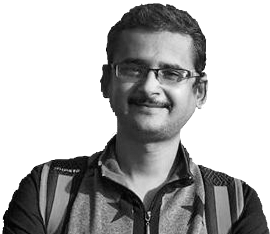
\includegraphics[width=.3\textwidth]{100-back/closeUp3.png}} &
\large{\textbf{Subhrendu Chattopadhyay} born in West Bengal, India. After completion of school education, he has completed the B.Tech from \emph{West Bengal University of Technology} (Now MAKAUT) in the area of
 \emph{Computer Science and Engineering} in 2010. He has completed M.Tech from the \emph{Department of Computer Science and Engineering}, \emph{Indian Institute of Technology Guwahati}, India in 2014, where he has continued working towards the PhD degree under the supervision of \textbf{Prof. Sukumar Nandi}. He has received \emph{TCS Research Scholar Fellowship} from Tata Consultancy Services, India for pursuing his PhD program. He has received best paper awards from \emph{IEEE ANTS 2013}, \emph{IEEE COMSNETS 2016} and best in session award from \emph{IEEE INFOCOM 2019}. His research interests include network architecture and management, wireless networks, distributed algorithms. He is interested to develop a cognitive network management architecture.}
\end{tabular}
\endcoverbio


%             \end{minipage}}
% \put(7,19){\transparent{0.8}\mycbox{black}{16cm}{4.75cm}} % background boxes
% \put(7,20){
\includegraphics[width=.2\linewidth]{100-back/iitg_white.png}}
%\put(25,28){\begin{minipage}{0.8\linewidth}\begin{flushleft}
%    \mbox{{\textbf {\color{coverfont} Department of Computer Science and Engineering}}}\vspace{.01\textheight}\\
%
%    \mbox{\large{\textbf {\color{coverfont} Indian Institute of Technology Guwahati}}}\vspace{.01\textheight}\\
%
%    \mbox{\Large{\textbf {\color{coverfont} Guwahati 781039, India}}}
%\end{flushleft}\end{minipage}}
%\end{overpic}
%\end{center}
%\restoregeometry
%\pagecolor{white}
%\color{black}
%============================================================================
% BackCoverPage
%===========================================================================
\chapter*{}
\thispagestyle{empty}
\begin{center}
\vspace{30ex}
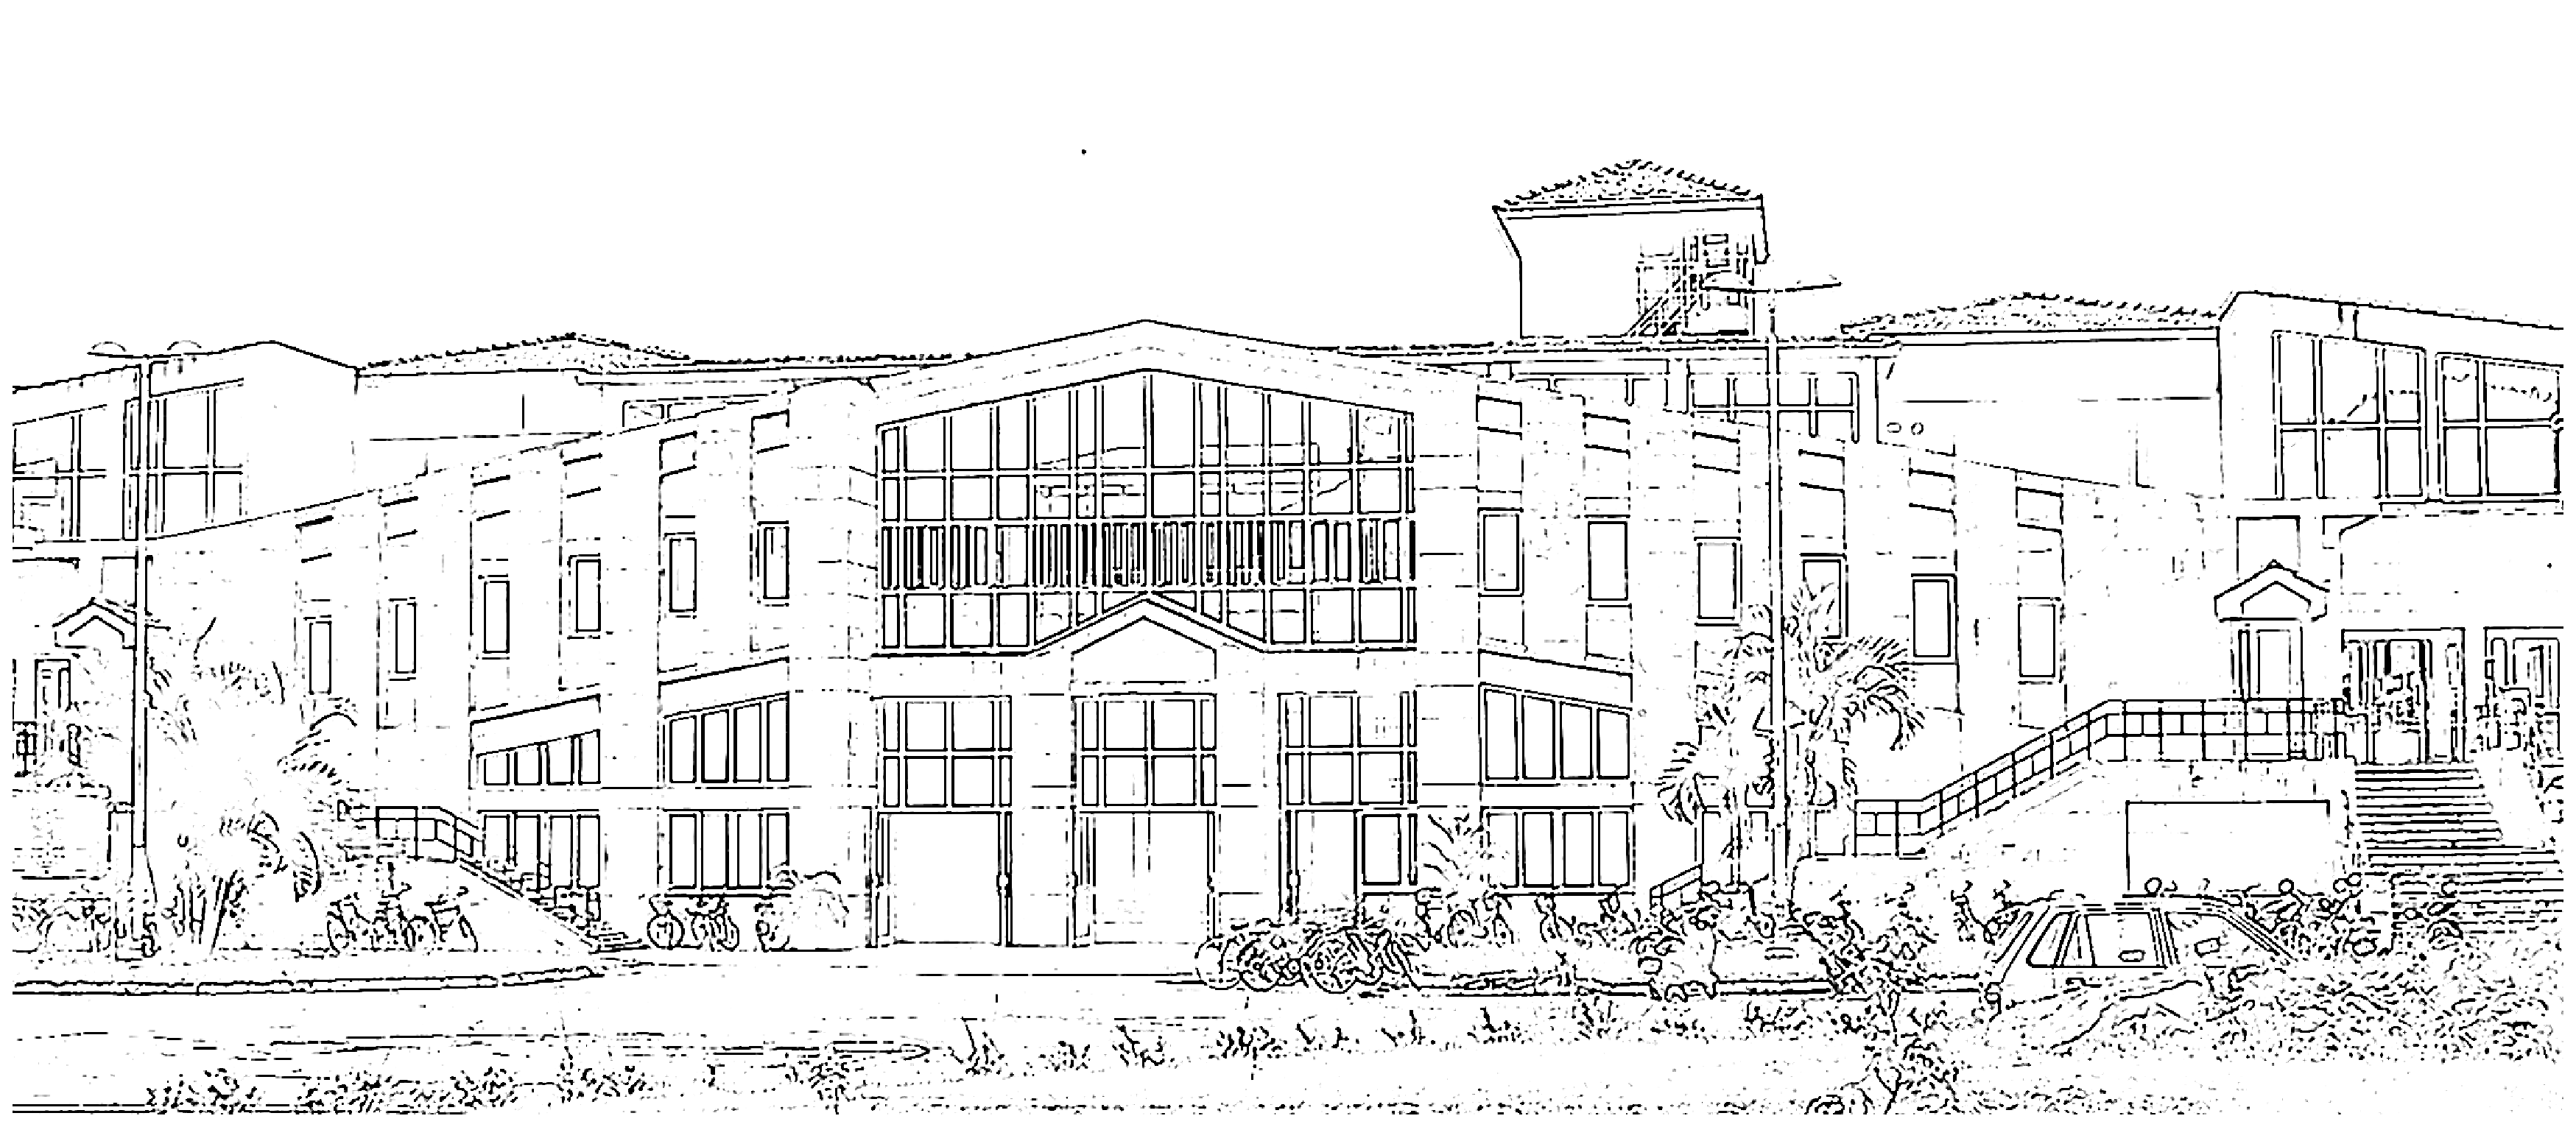
\includegraphics[width=\textwidth]{100-back/academic}
\begin{minipage}{0.2\linewidth}

\includegraphics[width=\textwidth]{100-back/IITG_logo.png}
\end{minipage}
\begin{minipage}{0.78\linewidth}
	\begin{flushleft}
    \textbf{Department of Computer Science and Engineering}\\
    \large{\textbf{Indian Institute of Technology Guwahati}}\\
    \Large{\textbf{Guwahati 781039, India}}
	\end{flushleft}
\end{minipage}
\end{center}

%  \includepdf[pages={4}]{C0_Cover.pdf}
%\printLog
%%%%%%%%%%%%%%%%%%%%%%%%%%%%%%%%%%%%%%%%%%%%%%%%%%%%%%%%%%%%%%%%%
%\jacket
\end{document}
